\section{Vorlesung 22.06.2016}

\subsection{olfaktorisches Lernen bei Drosophila}

\textcolor{red}{\textbf{Was passiert auf den ersten 16 Seiten??? Wie kann man das zusammenfassen???}}

\subsection{Interaktion multipler Gedächtnis-Systeme}
 - Lernen beruht auf einer Vielzahl von Mechanismen\\

\begin{itemize}
	\item Verschiedene Lernformen interagieren
	\begin{itemize}
		\item Ähnliche Lernsituation können auf unterschiedlichen
Prozessen basieren
		\item Die gleiche Lernsituation kann zu Beginn und Ende des Lernens auf unterschiedlichen Prozessen basieren
	\end{itemize}
	\item Gedächtnis das lange nach seinem Erwerb abgerufen wird ist oft unabhängig von der Struktur, mit der es erworben wurde („systemische Konsolidierung“; s. Patient H.M.).
	\item Erinnern, Vergessen, Neulernen und Umlernen sind komplexe Prozesse, die zum Teil ein Auflösen und eine „Re-Konsolidierung“ des Gedächtnisses zur Folge haben.
\end{itemize}

\textbf{Henry Gustav Molaison (Patient H.M.)}
\begin{itemize}
	\item Schwere anterograde Amnesie
	\item Partielle retrograde Amnesie
	\item Intaktes Arbeits-Gedächtnis
	\item Selektive Störung des deklarativen Gedächtnisses
	\item Patient zeigt normales motorisches Lernen
\end{itemize}

\textbf{Deklaratives Lernen: Hippocampus}\\
\textcolor{red}{\textbf{was kann man hier noch mitnehmen???}}

\subsection{Long Term Potentiation (LTP)}
 - Informationsspeicherung im Hippocampus ist vermutlich mit „Long Term Potentiation“ (LTP) verbunden

\begin{itemize}
	\item early LTP:
	\begin{itemize}
		\item ein Stimulus, kurze Phase von LTP
		\item dauert 1-3 Stunden an, keine neue Proteinsyntese
	\end{itemize}
	\item late LTP:
	\begin{itemize}
		\item 4 oder mehr Stimulus, persistente LTP-Phase
		\item dauert ca. 24 Stunden an, benötigt Protein und RNA-Synthese (cAMP-PKA-MAPK-CREB-1)
	\end{itemize}
\end{itemize}

\subsubsection{Postsynaptische Mechanismen}
 - der NMDA-Rezeptor als molekularer Koinzidenzdetektor
\begin{itemize}
	\item Nur Glutamat-Ausschüttung: der Kanal öffnet sich bleibt aber durch Mg verstopft
	\item Glu-Ausschüttung mit gleichzeitiger Depolarisation des postsynaptischen Neurons: Ca 2+ und Na + strömen ein.
\end{itemize}

$\Rightarrow$ Der intrazelluläre Anstieg des Ca 2+ führt zu einer lang anhaltenden Verstärkung der Synapse (Langzeit-Potenzierung; LTP)

\subsubsection{Präsynaptische Mechanismen}
 - NO ist ein gasförmiger Transmitter, der auch zur Präsynapse diffundiert (retrograder Transmitter) und dort über cGMP-abhängige Prozesse zu einer anhaltenden Verstärkung der Transmitterausschüttung führt.

\subsubsection{Übergang Kurz- zu Langzeitgedächtnis}
\textbf{ - Kurzzeit-Gedächtnis:} Verstellung der synaptischen Übertragung mit den vorhandenen Strukturen und Molekülen: Dendriten, Axone, Synapsen\\
\textbf{ - Langzeit-Gedächtnis:} Spezifische Aktivierung von Genen, Neubildung von Strukturen: Zellkern\\

\textbf{Beweis für eine LTP/Lern-Beziehung}
\begin{itemize}
	\item Mäuse mit NMDA-Rezeptoren \underline{unter} der normalen Funktion haben Lernschwäche
	\item Mäuse mit NMDA-Rezeptoren \underline{über} der normalen Funktion haben super Gedächtnis
	\item Drogen die LTP blocken, blocken lernen
	\item Drogen die LTP unterstützen, unterstützen lernen
\end{itemize}

\underline{Agonist} = aktiviert durch Besetzung eines Rezeptors die Signaltransduktion in der zugehörigen Zelle\\
\underline{Antagonist} = hemmt die Wirkung eines Agonisten, ohne selbst eine pharmazeutisch bedeutsame Wirkung auszulösen\\

AMPA:
\begin{itemize}
	\item Agonist: Glutamat, AMPA
	\item Antagonist: CNQX\footnote{\url{https://en.wikipedia.org/wiki/CNQX}}, NBQX\footnote{\url{https://en.wikipedia.org/wiki/NBQX}}
\end{itemize}

NMDA:
\begin{itemize}
	\item Agonist: Glutamat, NMDA
	\item Antagonist: APV\footnote{\url{https://en.wikipedia.org/wiki/AP5}}, 
\end{itemize}

Test für Gedächtnisbildung - \textbf{the Morris water maze}\footnote{\url{https://de.wikipedia.org/wiki/Morris-Wasserlabyrinth}}\\

\textbf{Das lineare Modell der Gedächtnisbildung}\\
 - Funktioniert unser Gehirn tatsächlich wie eine Festplatte?

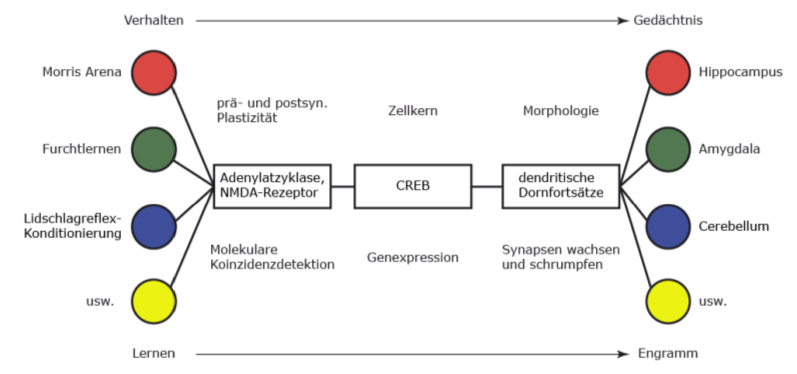
\includegraphics[width=1\textwidth]{lectures/160622/pix/memory_genesis.png}